%ajouter draft pour voir débordement

%%%%%

\documentclass[12pt,french]{article}


\usepackage[utf8]{inputenc}
\usepackage[T1]{fontenc}
\usepackage{lmodern}
%règles mes marges et format papier
\usepackage{geometry} %modif marge et formet
\geometry{left=3cm,right=2cm,top=2.5cm,bottom=2.5cm}
\usepackage{amsmath, amssymb, amsthm}
\usepackage{fancyhdr} %pour les entêtes et bas de page
\usepackage{lastpage} %pour numéroter les pages charge la derniere page
\usepackage{graphicx} %pour inclure des img
\usepackage{dsfont}
\usepackage{float} %pour le placement des figures
\usepackage{hyperref} %pour mettre des liens hypertext
\usepackage{calc} %permet de calculer les marges pour encadrer les textes
\usepackage{color, xcolor} %gère les couleurs
\usepackage{babel}
\usepackage{listings} %pour afficher le code annexe
% Ajout du package glossaries 
\usepackage{glossaries} 
% Création du glossaire 
\makeglossaries

%pour afficher le code de manière esthétique
\lstset{
  aboveskip=3mm,
  belowskip=-2mm,
  backgroundcolor=\color{white},
  basicstyle=\footnotesize,
  breakatwhitespace=false,
  breaklines=true,
  captionpos=b,
  commentstyle=\color{red},
  deletekeywords={...},
  escapeinside={\%*}{*)},
  extendedchars=true,
  framexleftmargin=16pt,
  framextopmargin=3pt,
  framexbottommargin=6pt,
  frame=tb,
  keepspaces=true,
  keywordstyle=\color{blue},
  language=C,
  literate=
  {²}{{\textsuperscript{2}}}1 {⁴}{{\textsuperscript{4}}}1
  {⁶}{{\textsuperscript{6}}}1
  {⁸}{{\textsuperscript{8}}}1
  {€}{{\euro{}}}1 {é}{{\'e}}1 {è}{{\`{e}}}1 {ê}{{\^{e}}}1 {ë}{{\¨{e}}}1
  {É}{{\'{E}}}1 {Ê}{{\^{E}}}1 {û}{{\^{u}}}1 {ù}{{\`{u}}}1 {â}{{\^{a}}}1
  {à}{{\`{a}}}1 {á}{{\'{a}}}1 {ã}{{\~{a}}}1 {Á}{{\'{A}}}1 {Â}{{\^{A}}}1
  {Ã}{{\~{A}}}1 {ç}{{\c{c}}}1 {Ç}{{\c{C}}}1 {õ}{{\~{o}}}1 {ó}{{\'{o}}}1 
  {ô}{{\^{o}}}1 {Õ}{{\~{O}}}1 {Ó}{{\'{O}}}1 {Ô}{{\^{O}}}1 {î}{{\^{i}}}1
  {Î}{{\^{I}}}1 {í}{{\'{i}}}1 {Í}{{\~{Í}}}1,
  morekeywords={*,...},
  numbers=left,
  numbersep=10pt,
  numberstyle=\tiny\color{black},
  rulecolor=\color{black},
  showspaces=false,
  showstringspaces=false,
  showtabs=false,
  stepnumber=1,
  stringstyle=\color{gray},
  tabsize=4,
}

%Personalisation En tête
\pagestyle{fancy}
\renewcommand\headrulewidth{1pt}
%\setlength{\headheight}{2.5cm}

\fancyhead[L]{Projet de 60 heures}
\fancyhead[C]{
\includegraphics[scale=0.22]{header.png}}
\fancyhead[R]{2022 - 2023}


\renewcommand\footrulewidth{1pt}
\fancyfoot[L]{BALLEJOS Lilian}
\fancyfoot[C]{\thepage/\pageref{LastPage}}
\fancyfoot[R]{CHARPIN Etienne}
%Fin personalisation En Tête

%table des matieres
\renewcommand\thesection{\Roman{section}}
\renewcommand\thesubsection{\arabic{subsection}}
\renewcommand\thesubsubsection{\thesubsection.\arabic{subsubsection}}


\begin{document}

\newgeometry{margin=2.5cm}
\begin{titlepage} %page d'acceuil

  
  \begin{center}
  	
\includegraphics[scale=0.35]{isima.png}
  \end{center}
  
  %\hspace*{\stretch{1}}%espace horizontal entre les 2 images
  %
\includegraphics[scale=0.25]{deco.png}
  
  \vspace*{3cm} %espace de 2.5cm en dessous des images
  
  \hrule
  
  \begin{center}
  	\large
  	Rapport d'élève ingénieur
  	
  	Projet de 2ème année
  	
  	Filière: Génie Logiciel et Systèmes Informatiques
  	
  	\huge
  	\textbf{Projet Fullstack de Révision de Parole}
  \end{center}

\hrule
  
  \vspace*{1.8cm} 
  
  \begin{center}
 
  	
  \Large Présenté par : \textbf{BALLEJOS Lilian et CHARPIN Etienne}
  
   \end{center}

\vspace*{7cm}
  
  
  
  
  	\begin{minipage}{.45\linewidth}
  		\begin{flushleft}
  			\textbf{Responsable ISIMA: YON Loic}
  			
  			\textbf{Soutenance : Jeudi 23 Mars}
  		\end{flushleft}
  	\end{minipage}
  	\hfill
  	\begin{minipage}{.45\linewidth}
  		\begin{flushright}
  			\textbf{Projet de 60 heures}
  			
  			\textbf{Année Scolaire 2022 - 2023}
  		\end{flushright} 
  	\end{minipage}
  	
  	\vspace*{2cm} 
  	
    Campus des Cézeaux. 1 rue de la Chebarde. TSA 60125. 63178 Aubière CEDEX
    	

\end{titlepage}

\restoregeometry



\normalsize\tableofcontents %place la table des matières

\newpage

\section{Contexte du projet}

\subsection{Introduction au Full Stack}

Pour commencer l'explication du projet, nous allons faire une brève introduction au \textbf{Full Stack}.

\medskip

Lors d'un projet informatique de développement web, l'architecture du logiciel va être séparée en plusieurs parties distinctes : la partie côté serveur dite le "back", puis la partie côté utilisateur dite le "front".

\medskip

La partie front va être chargée sur le moteur de recherche de l'utilisateur et donc le code sera disponible et exploitable par n'importe quel utilisateur du site web (par exemple, le code HTML ainsi que le code Javascript).

\medskip

À l'inverse, la partie back va gérer tous les comportements communs que l'on doit garder côté serveur (interagir avec la base de données, contacter une API...).

\medskip

Lorsqu'on parle de Full Stack, on parle donc du développement de ces deux aspects. D'où le terme Full Stack qui peut se comprendre comme "travailler tous les aspects du projet".

\medskip

Dans ce projet, nous allons vous montrer comment nous avons implémenté un projet Full Stack avec un back en Node.js à l'aide du module "Express" et un front à l'aide du framework Angular.

\begin{figure}[H]
	\centering
	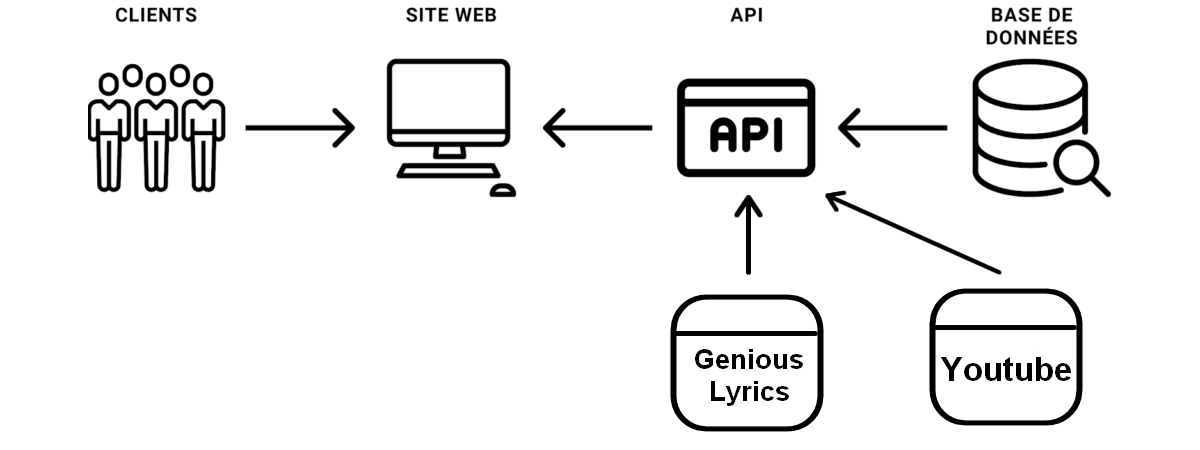
\includegraphics[scale=0.4]{fullstack.png}
	\caption{Organigramme de notre Application Fullstack}    
\end{figure}

\section{Réalisation et conception}

\subsection{Nos choix}

\subsubsection{Le Back de notre site}

Pour la partie back de notre projet, nous avons choisi de prendre Node.js avec le module "Express".

\medskip

L'un de nous avait déjà travaillé sur cette technologie, donc cela permettait pour l'un, de ne pas partir de zéro et d'améliorer ses connaissances, et pour l'autre de découvrir une nouvelle technologie possiblement très utile pour notre filière de développement à l'ISIMA.

\medskip

De plus, Node.js est une technologie plus récente que d'autres langages qui peuvent gérer le côté serveur (comme PHP, par exemple). Ainsi, le module Express que nous utilisons est toujours maintenu à jour.

\medskip

Avec Express, nous pouvons en quelques minutes implémenter une API assez facilement et parfaitement fonctionnelle. Cela nous a permis de bien scinder la partie front et back de notre projet.
Nous pouvons par exemple citer l'exemple de PHP, où la partie serveur et client est parfois mélangée dans les mêmes fichiers.

Ici, nous avons le back dans un dossier et le front dans un autre, et ces deux aspects sont parfaitement indépendants ! On peut, par exemple, lancer le back pour faire des tests dessus sans toucher au front.

La partie front va pouvoir communiquer avec la partie back à l'aide de requêtes envoyées à celui-ci, auxquelles il va répondre.

\bigskip

Au niveau de l'organisation de notre back, nous avons séparé celui-ci en différentes couches.

\medskip

\begin{itemize}
	\item \textbf{Couche "Controller"} : réceptionne les requêtes et appelle les fonctions nécessaires en fonction de la demande. Répond ensuite aux requêtes. Elle correspond au fichier \textit{listen.js}.
	\item \textbf{Couche "Business"}: effectue tous les calculs de notre API, on implémente dans celle-ci toutes les fonctions nécessaires au bon fonctionnement de l'API (communication avec d'autres API, création de trou à compléter dans les paroles etc...). Elle correspond à tous les fichiers \textit{gestion\_*.js} sauf "\textit{gestion\_database.js}"
	\item \textbf{Couche "Base de donnée"}: effectue toutes les requêtes à la base de donnée et renvoie les données récupérées. Elle est appelées par la couche business. Elle correspond au fichier \textit{gestion\_database.js}.
	
\end{itemize}

\bigskip

\begin{figure}[H]
	\centering
	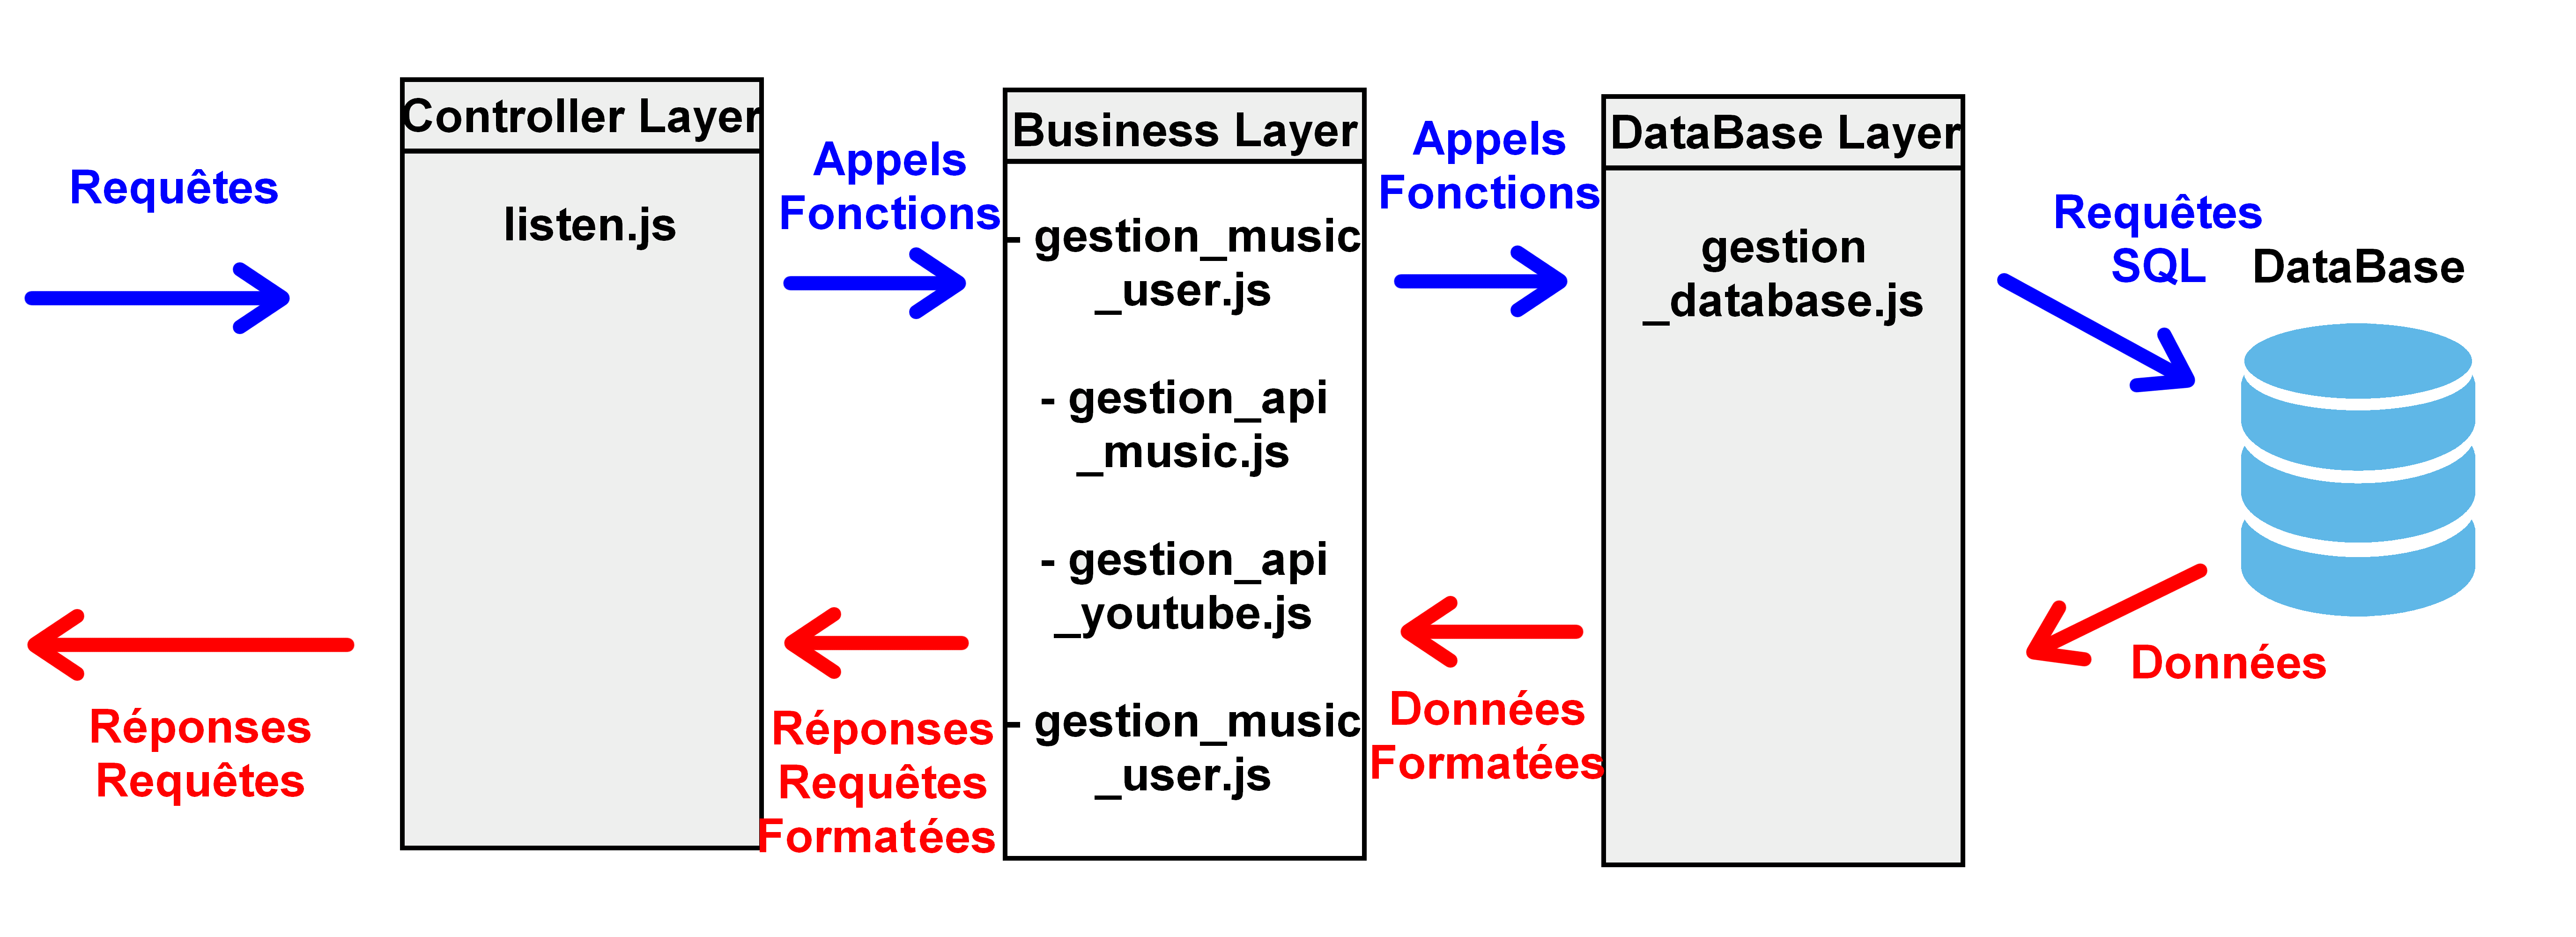
\includegraphics[scale=0.1]{api_couche.png}
	\caption{
	L'organisation de l'API}    
\end{figure}

\bigskip

Pour démarrer notre API, nous lançons le fichier \textbf{server.js} qui positionne notre API sur le port souhaité de notre machine. Ensuite, il se connecte à la base de données. Enfin, une fois que tout cela est effectué, nous activons les différents contrôleurs de l'API et nous sommes prêts à recevoir des requêtes !

\begin{figure}[H]
	\centering
	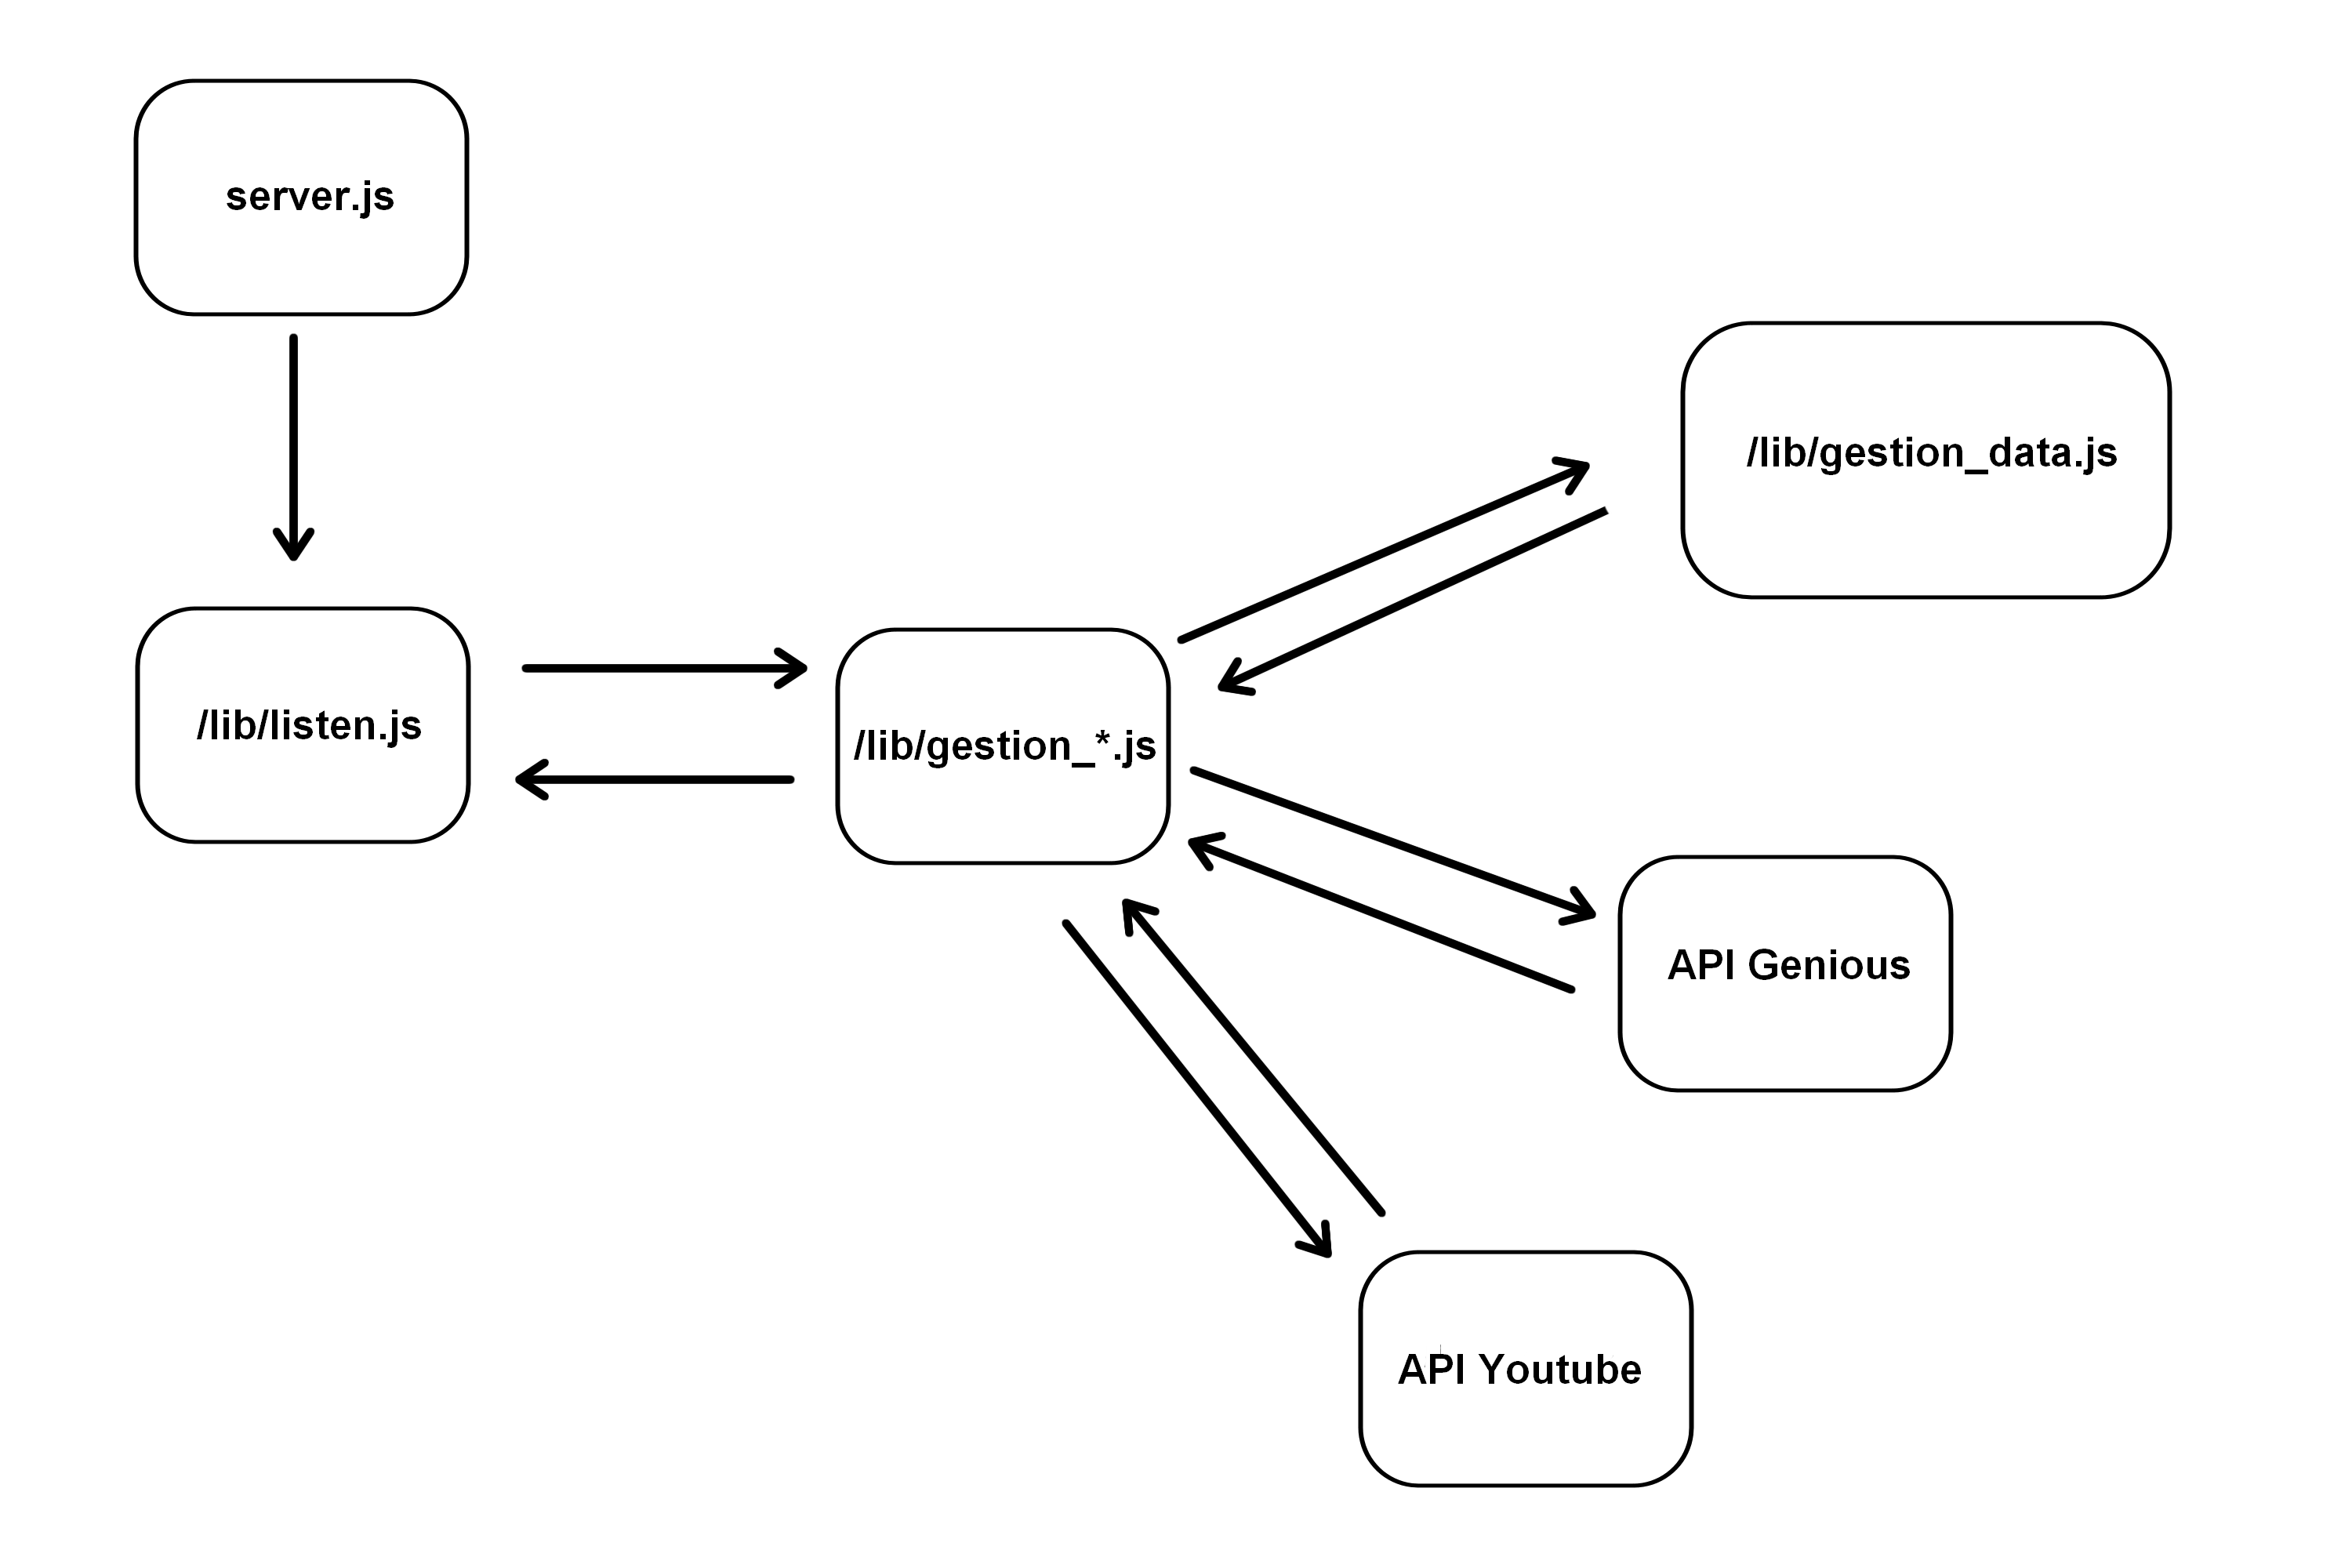
\includegraphics[scale=0.16]{api.png}
	\caption{Architecture de l'API}
\end{figure}

\medskip

On peut voir ici que nous communiquons avec d'autres API publiques ! Nous vous expliquerons cela plus en détail par la suite.

\subsubsection{Le Front}

Pour la partie Front, nous avons choisi d'utiliser un Framework car ces technologies sont plus évoluées pour effectuer des comportements complexes.

\medskip

L'un des gros avantages de ces technologies est de pouvoir séparer notre application en plusieurs composants que nous allons pouvoir faire interagir les uns avec les autres ou encore inclure les uns dans les autres ! Cela permet de structurer plus proprement et efficacement une application.

\medskip

De plus, les Framework sont des outils très puissants avec de nombreuses fonctionnalités pré-implémentées. Cela nous permet de ne pas avoir besoin de réinventer la roue et de nous concentrer sur nos propres implémentations.

\medskip

Ainsi, nous avons hésité entre le Framework Angular et ReactJS qui sont les plus courants et les plus utilisés de nos jours. Notre choix s'est finalement porté sur Angular car nous étions familiers avec ce Framework grâce à des projets personnels. 

\medskip

L'avantage de ce Framework est qu'il utilise nativement Typescript dans la version que nous utilisons, ce qui permet de créer des applications plus claires en typant les variables et les objets utilisés. De plus, chaque composant généré est composé d'un fichier HTML, un fichier SCSS et un fichier Typescript, ce qui permet de bien séparer les trois aspects importants du front qui sont respectivement, dans l'ordre, le corps d'une page, son style et son comportement.

\bigskip

En plus d'Angular, nous avons utilisé le Framework \textbf{Bootstrap} pour avoir des éléments graphiques classes et au goût du jour. Par exemple, notre barre de navigation a été stylisée grâce à ce Framework.

De plus, nous avons utilisé \textbf{PrimeNg} qui est une bibliothèque de composants Angular. Nous y retrouvons plein d'éléments déjà créés très pratiques comme des dossiers (que nous avons utilisés pour la partie utilisateur) ou encore des boutons déjà stylisés.


\subsubsection{Choix des APIs}

Nous avons dû utiliser pour ce projet deux APIs publiques de deux entreprises différentes.

\medskip

Ces APIs nous permettent de récupérer des informations, comme par exemple des paroles de musique, et nous ont été très utiles. Pour chacune d'elles, nous avons dû nous inscrire sur le site de la documentation afin d'obtenir un token pour communiquer avec elles.

\paragraph{Gestion des lecteurs vidéos avec paroles de musique \\\\}

La première est l'API de \textbf{Youtube} de l'entreprise \textbf{Google}. Nous lui demandons, via une requête, le meilleur résultat pour une recherche avec les mots clés "\textit{nom musique}" + "\textit{nom artiste}" + "lyrics".

L'API nous répond en envoyant une liste des 5 vidéos sur sa plateforme qui correspondent le mieux à la recherche et nous renvoyons le résultat numéro 1 à la partie utilisateur afin d'afficher le bon URL dans le lecteur.

\paragraph{Récupération des paroles de musique \\\\}

Notre second objectif était de trouver une API qui pourrait nous fournir les paroles de musique et qui couvre donc un très grand nombre d'entre elles.

\medskip

Nous nous sommes tout d'abord penchés sur l'API \textbf{ChartLyrics}, puis nous nous sommes rendus compte que celle-ci était trop incomplète. L'API étant américaine, nous avions très peu de musique française dessus, ce qui est très dommage au vu de notre projet.

\medskip

Ainsi, nous nous sommes ensuite penchés sur une autre API d'un site très connu qui couvre de très nombreuses musiques très diversifiées : \textbf{Genius Lyrics}.

Le problème de cette API est que, dû à des problèmes de droits sur les paroles de musique (gérés en France par la \textbf{SACEM}), nous ne pouvons pas obtenir les paroles de musique directement via des requêtes.

La solution est la suivante : l'API nous fournit le lien vers la page web du site \textbf{Genius Lyrics}. Nous récupérons ce lien et, grâce au Web scraping, nous arrivons à récupérer les paroles.

Dans l'ordre, la méthode pour récupérer les paroles d'une musique est donc la suivante :

\medskip

\begin{itemize}
	\item On contacte l'API Genius Lyrics et on lui demande l'URL de la page du site qui contient les paroles.
	\item On aspire ensuite tout le code HTML de la page web du site.
	\item Les paroles étant toujours dans la même balise HTML, on les récupère tout en ignorant le reste du contenu de la page.
	\item Enfin, on formate les paroles pour qu'elles soient plus adaptées à de l'apprentissage.
\end{itemize}

\medskip

\subsection{Le déroulement du projet}

Notre façon de travailler était comparable à une méthode agile de développement, c'est-à-dire que nous avons séparé le projet en différentes parties comme vous l'avez vu plus tôt (partie parole, partie utilisateur, etc.). À chaque partie du projet, nous avons effectué un sprint durant lequel nous suivions toujours le même schéma de travail :

\begin{itemize}
	\item Nous avons implémenté ou modifié la base de données.
	\item Nous avons relié la partie serveur (back) du projet à la base de données.
	\item Nous avons implémenté les fonctionnalités nécessaires côté serveur.
	\item Nous avons relié la partie utilisateur (front) à la partie serveur (back).
	\item Nous avons testé la fonctionnalité implémentée.
\end{itemize}

\begin{figure}[H]
	\centering
	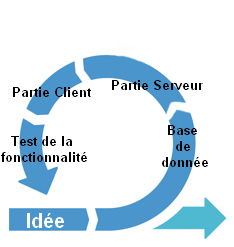
\includegraphics[scale=1]{agile.png}
	\caption{Les différentes étapes d'ajout d'une fonctionnalité}
\end{figure}

Finalement, nous avons effectué à la fin une embellissement de la partie utilisateur (front) car il est très important d'avoir une interface utilisateur très agréable d'utilisation pour faciliter l'interaction avec notre application.

Maintenant, voyons en détail ce que chaque partie d'un sprint impliquait.

\subsubsection{Exemple complet d'un Sprint}

\paragraph{Modification de la base de données \\\\}

À chaque nouveau sprint, nous regardions tout d'abord si une modification de la base de données était nécessaire.

Si c'était le cas, nous reconstruisions notre base de données en ajoutant les nouvelles tables et colonnes nécessaires.

Cela impliquait de modifier le script \textbf{setupDatabase.js} pour que nous ayons chacun de notre côté, en local, exactement la même base de données.

Lorsque cela était fait, nous effectuions chacun de notre côté des tests en local sur nos machines afin de vérifier que nos bases de données avaient le même comportement.

\paragraph{Mise en lien de la base de données avec notre partie serveur \\\\}

Ensuite, on reliait la base de données à la partie serveur.

\medskip

Le principe est le suivant : on créait des requêtes SQL qui permettent de récupérer les données dont on a besoin pour les futures implémentations.

On incluait ensuite ces requêtes dans le code JavaScript de notre back dans le fichier \textit{gestion\_database.js}.

Enfin, on créait dans la "couche business" toutes les fonctions nécessaires pour formater les données comme il nous faut.

C'est durant cette partie aussi que l'on a créé les fonctions qui envoient des requêtes HTTP à des APIs si nécessaire. Comme avec la base de données, après avoir reçu les données, on les formatées afin de mieux les exploiter dans le front.

\paragraph{Mise en lien de la partie serveur avec la partie utilisateur \\\\}


Au final, il ne nous restait plus qu'à créer côté client les nouveaux composants Angular nécessaires pour implémenter la nouvelle fonctionnalité. Ensuite, on avait juste à créer les requêtes à envoyer à notre partie serveur pour récupérer les éléments nécessaires côté client.

\subsubsection{Nos différents Sprints effectués}

Nous avons effectué ainsi 3 sprints durant le développement de notre application web.

\begin{itemize}
	\item Le développement de la partie entrainement avec les paroles
	\item Le développement de la partie inscription/connexion
	\item Le développement de la partie stockage des musiques avec les dossiers utilisateurs
\end{itemize}


\subsubsection{Embellissement du front}

Au départ, nous avons cherché à développer une application fonctionnelle sans nous pencher de trop sur l'apparence. Nous avons essayé de développer toutes les fonctionnalités que nous voulions ajouter en nous assurant que celles-ci ne présentaient aucun bug.

\medskip

Après nous être assurés que tout fonctionnait comme nous le souhaitions, nous avons décidé à la toute fin d'embellir le front. Nous avons pour cela utilisé nos connaissances en CSS ainsi qu'en Bootstrap.

\medskip

Ayant quelques notions d'IHM (interface homme machine), nous savons que l'apparence d'un site web est une étape primordiale du développement logiciel. En effet, il ne faut pas utiliser, par exemple, des contrastes de couleur qui pourraient gêner certaines personnes comme les daltoniens.

De plus, chaque élément du site doit être intuitif et c'est ainsi que nous avons essayé de faire des fonctionnalités très simples d'utilisation (boutons simples, pas trop de détails, etc.).

\begin{figure}[H]
	\centering
	\begin{minipage}{.5\textwidth}
		\centering
		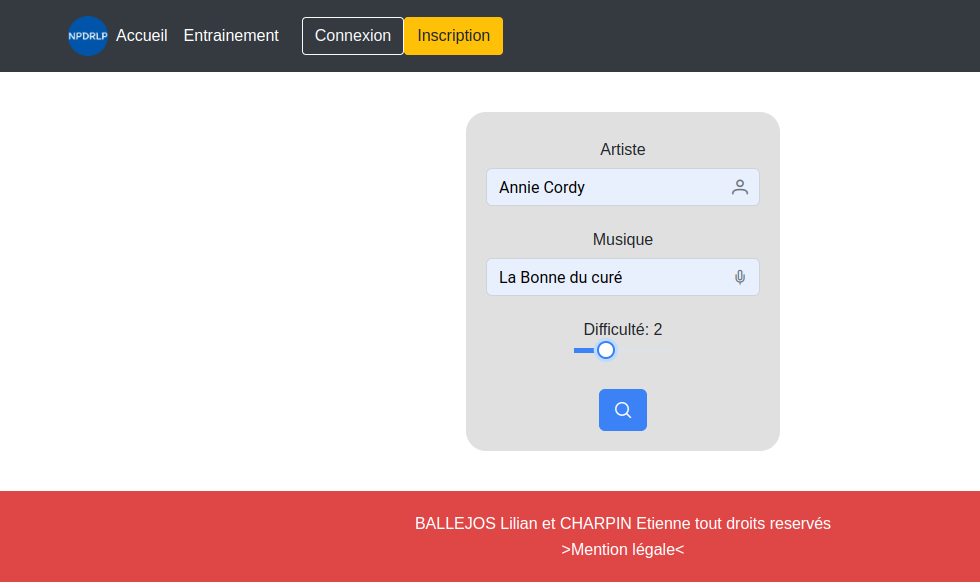
\includegraphics[scale=0.25]{avantfront.png}
	\end{minipage}%
	\begin{minipage}{.5\textwidth}
		\centering
		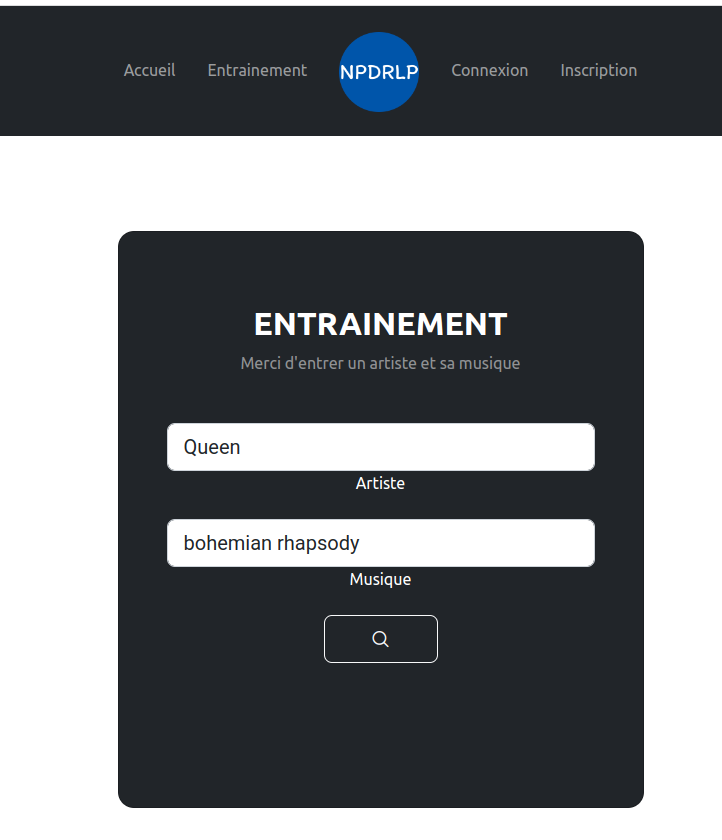
\includegraphics[scale=0.25]{apresfront.png}
	\end{minipage}
	\caption{Avant / Après de l'apparence de la partie client}
\end{figure}

\section{Résultats et discussions}

\subsection{Prise en Main de l'Application Web}

\subsubsection{Comment lancer l'Application Web}

Nous n'avons pas exporté notre projet car il est encore en phase de développement. Pour lancer notre application sur une machine, il faut suivre quelques étapes.

\paragraph{Installation et configuration (à faire une fois) \\\\}

Tout d'abord, il vous faudra installer quelques logiciels :

\begin{itemize}
	\item \textbf{mysql} : Pour la gestion de la base de données.
	\item \textbf{node} ainsi que son package manager \textbf{npm} : Pour lancer la partie serveur et la partie utilisateur.
\end{itemize}

\bigskip

Ensuite, vous pouvez trouver notre projet sur GitHub à ce lien :

\textbf{\href{https://github.com/LIlianHub/projetZZ2-NPDRLP}{https://github.com/LIlianHub/projetZZ2-NPDRLP}}

\bigskip

Après avoir installé le projet sur votre machine, il va falloir aller dans les dossiers "\textit{backend-api}", "\textit{frontend-angular}" et "\textit{setupDataBase}" et exécuter \textbf{dans ces 3 dossiers} la commande \textbf{npm i}, qui va permettre d'installer les dépendances nécessaires.

\bigskip

Une fois cela fait, lancez \textbf{mysql} et créez une nouvelle base de données nommée \textbf{npdrlp} en entrant la commande \textbf{CREATE DATABASE npdrlp}.

\bigskip

Ensuite, rendez-vous dans le dossier \textit{setupDataBase} et exécutez \textbf{node setup.js} afin de lancer la configuration de la base de données.

\paragraph{Lancer l'application \\\\}

Pour lancer l'application et la tester, il vous suffit de suivre ces deux étapes :

\begin{itemize}
	\item Dans \textit{backend-api}, entrez la commande \textbf{node server.js}.
	\item Dans \textit{frontend-angular}, entrez la commande \textbf{ng serve}.
\end{itemize}

Une fois cela fait, vous pouvez accéder à notre projet en local à cette adresse :

\textbf{\href{http://localhost:4200}{http://localhost:4200}}

\subsubsection{Arrivée sur le site}

En arrivant sur le site, vous arrivez sur une page d'accueil défilante qui vous informe du concept de notre application, de qui nous sommes et de nombreuses autres informations.

Nous pouvons si nous le souhaitons changer le code source du site web afin de rajouter des éléments à l'accueil, cela sans difficulté !

\bigskip

En haut de la page, vous pouvez voir les différentes fonctionnalités de notre site web proposées dans le header. Vous avez la possibilité d'aller à l'accueil (là où nous sommes actuellement) mais aussi dans la partie entraînement. Vous pouvez également vous inscrire ou, si cela est déjà fait, vous connecter !

Le header va changer en fonction de si vous êtes connecté ou non. Si vous êtes connecté, au lieu de la possibilité de vous inscrire ou de vous connecter, vous aurez la possibilité d'aller à votre menu utilisateur ou de vous déconnecter.

\begin{figure}[H]
	\centering
	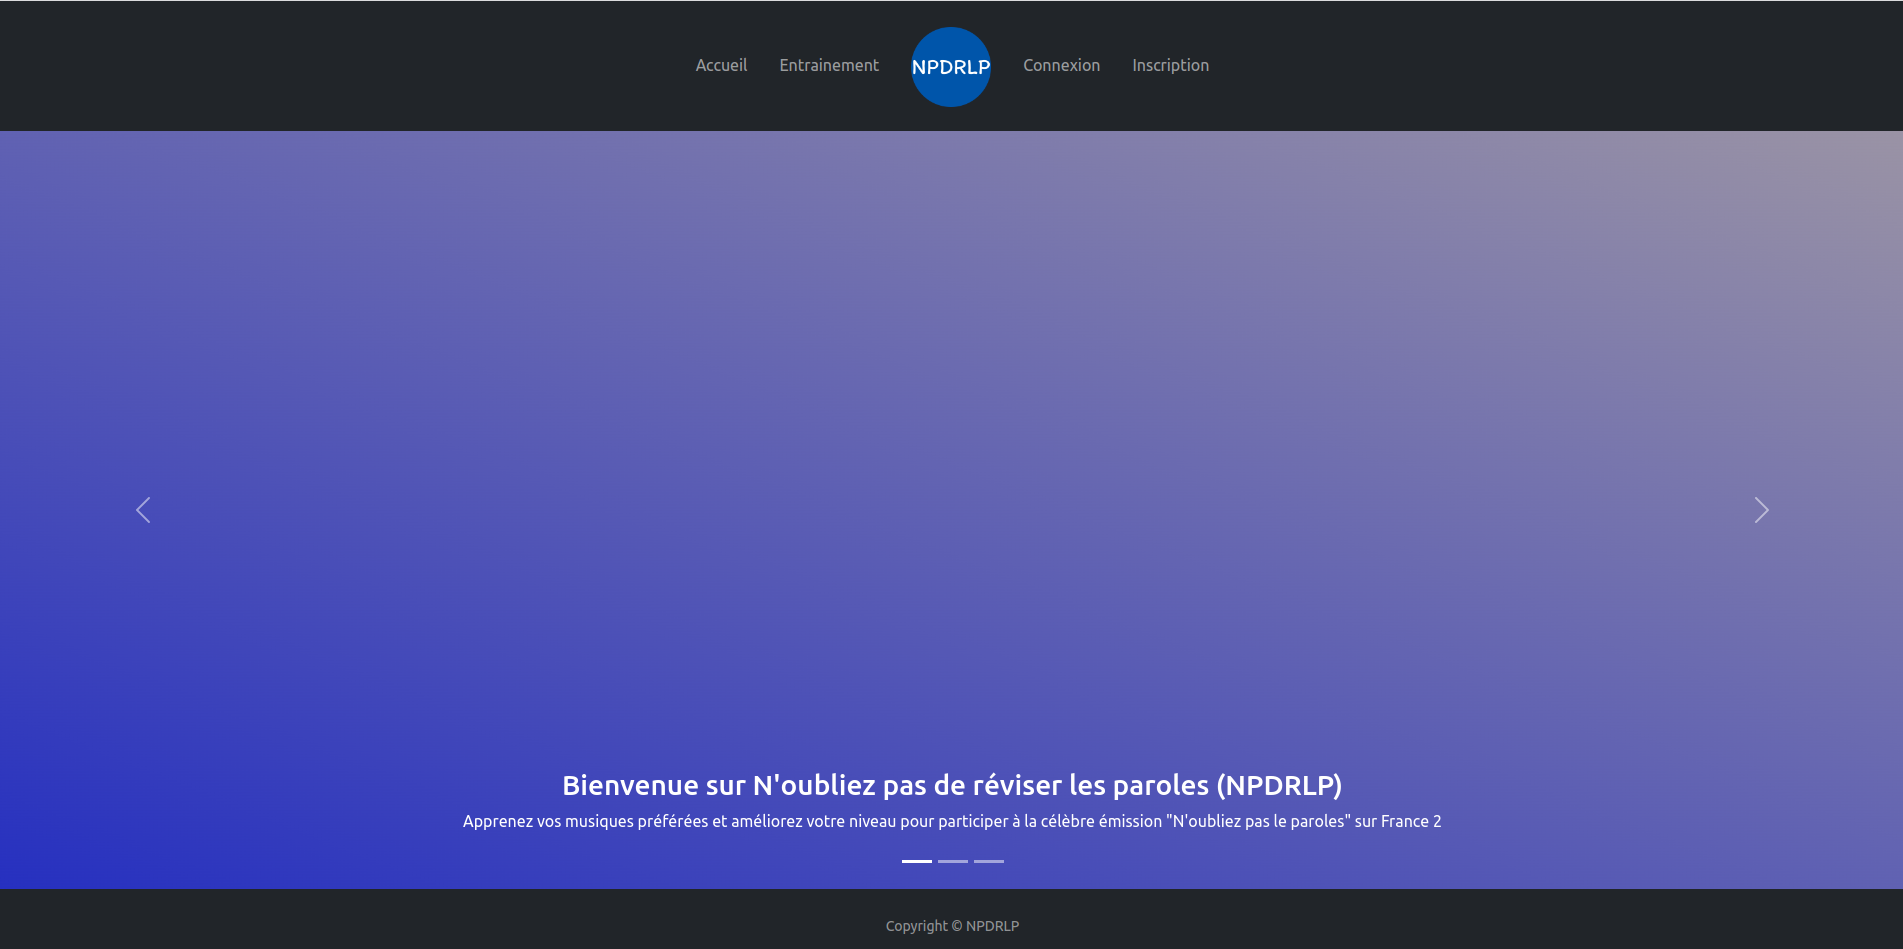
\includegraphics[scale=0.25]{accueil.png}
	\caption{La page d'accueil de notre site web.}
\end{figure}


\subsubsection{Partie Entrainement}

En arrivant dans la partie entraînement, un formulaire vous demande de renseigner à la fois le nom de l'artiste ainsi que la musique que vous souhaitez apprendre.

\begin{figure}[H]
	\centering
	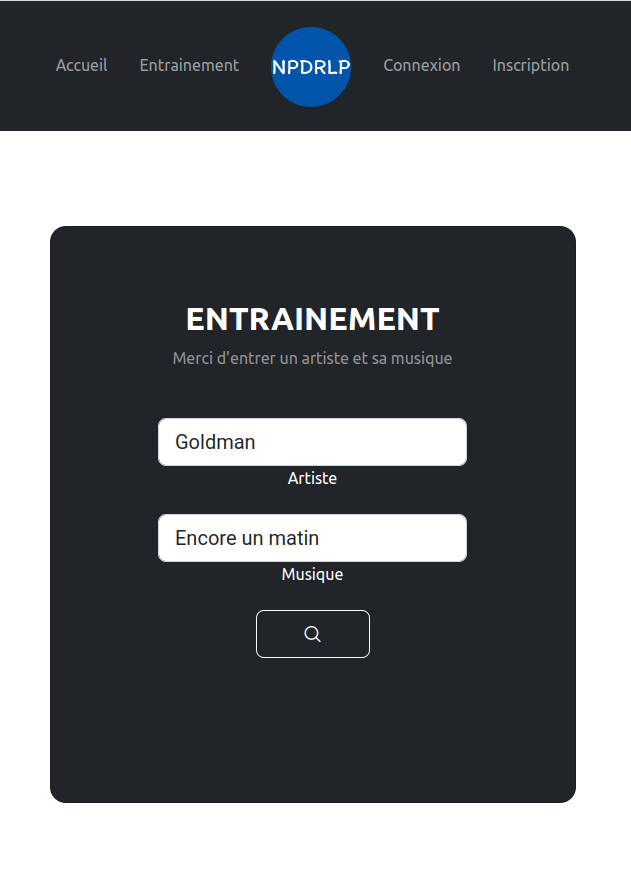
\includegraphics[scale=0.25]{rechercheparole.png}
	\caption{Formulaire de recherche de paroles}
\end{figure}

Si vous renseignez quelque chose de faux ou erroné, l'application affichera un message d'erreur vous informant que les paroles n'ont pas pu être trouvées.

Si les informations renseignées sont correctes, alors l'intégralité des paroles de la musique est affichée sur votre écran. En dessous de celles-ci, vous trouverez un lecteur YouTube avec une vidéo de la musique recherchée.

\begin{figure}[H]
	\centering
	\begin{minipage}{.5\textwidth}
		\centering
		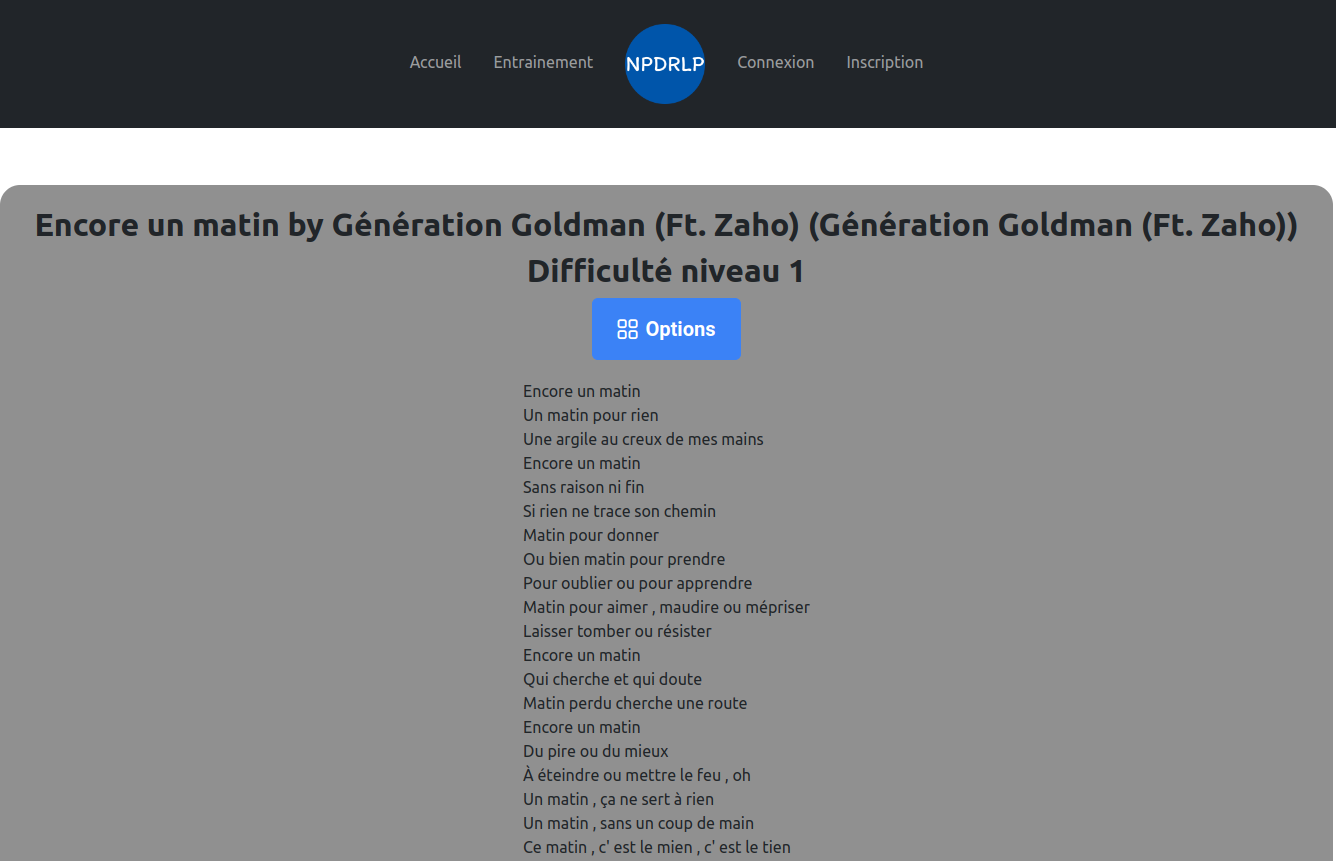
\includegraphics[scale=0.15]{parole.png}
	\end{minipage}%
	\begin{minipage}{.5\textwidth}
		\centering
		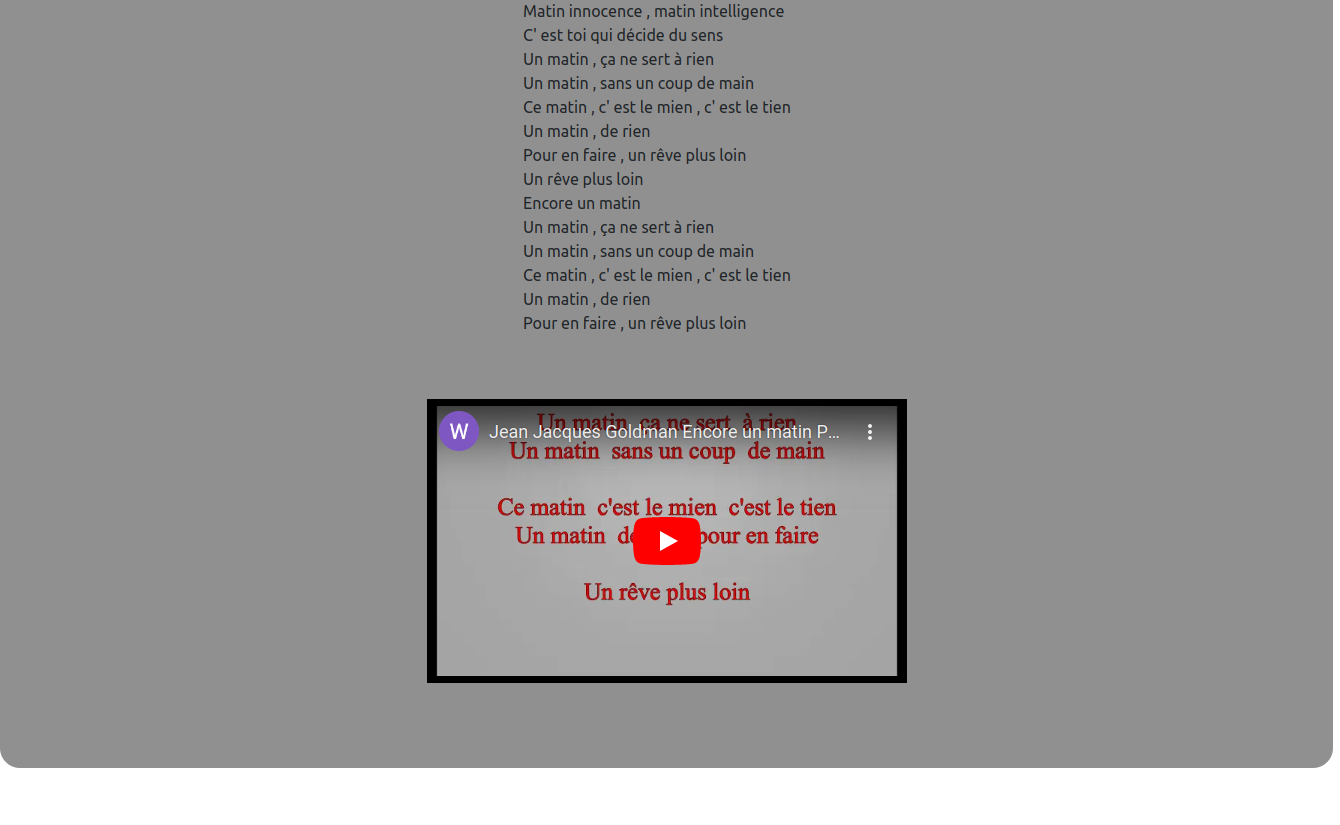
\includegraphics[scale=0.15]{ytbparole.png}
	\end{minipage}
	\caption{Affichage des paroles dans le mode entraînement}
\end{figure}

Enfin, nous trouvons au-dessus des paroles un bouton "Options" sur lequel nous pouvons cliquer. Lors du clic sur celui-ci, un menu apparaît sur la gauche avec deux fonctionnalités :

\begin{itemize}
	\item Sauvegarder la musique dans un dossier
	\item Changer la difficulté
\end{itemize}

\bigskip

\begin{figure}[H]
	\centering
	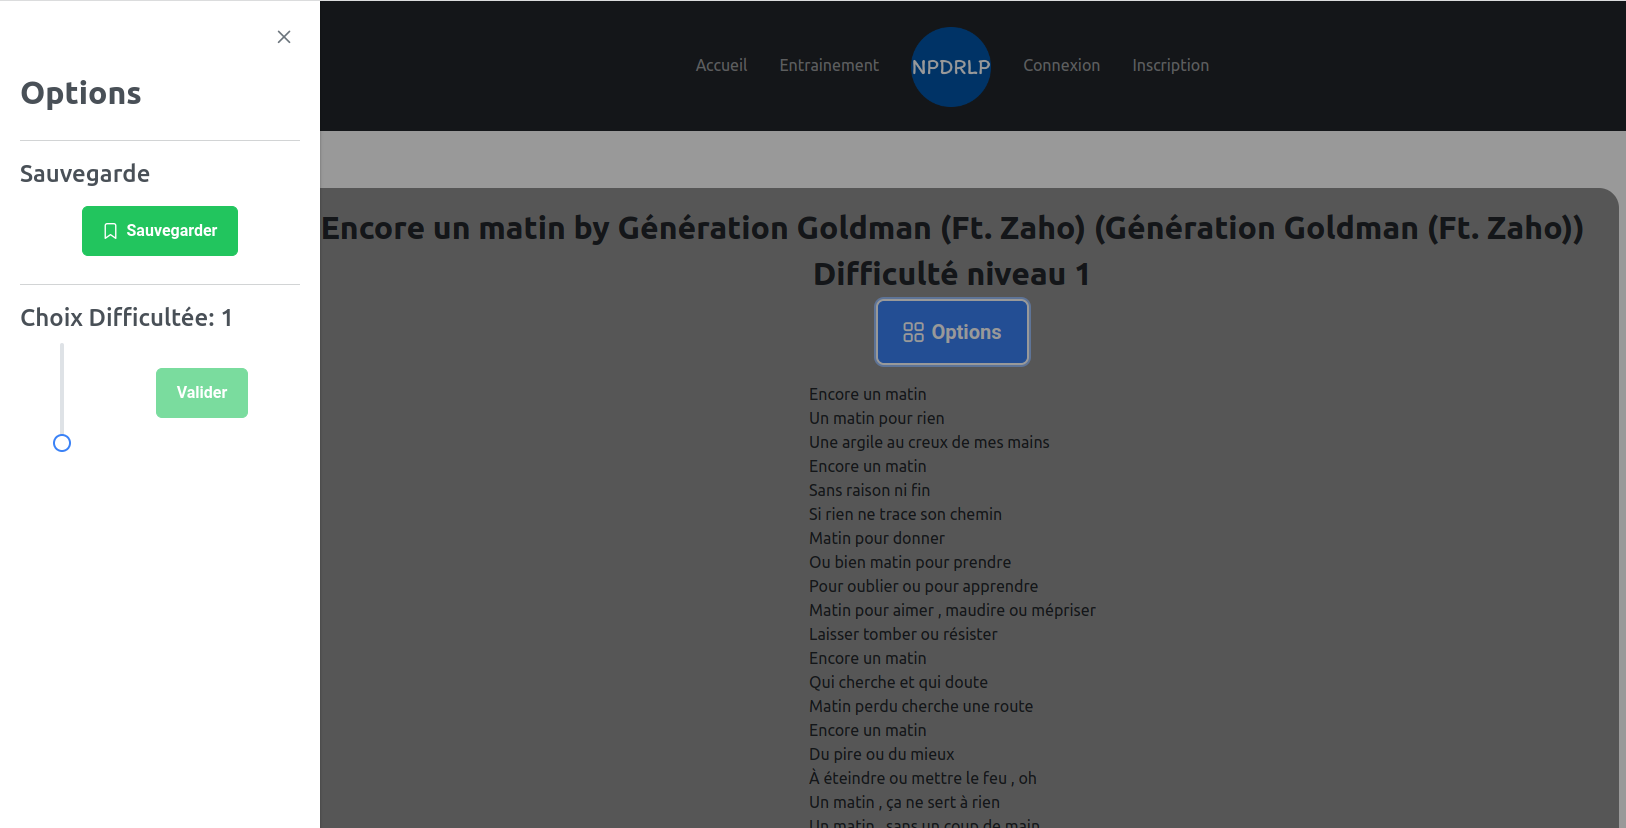
\includegraphics[scale=0.25]{optionparole.png}
	\caption{Options du mode entraînement}
\end{figure}

\paragraph{Sauvegarder la musique dans un dossier \\\\}

Lorsque vous cliquez sur le bouton "Sauvegarder la musique", deux possibilités s'offrent à vous. Si vous n'êtes pas connecté, nous vous informons qu'il faut que vous vous connectiez si vous souhaitez sauvegarder une musique. Sinon, une liste déroulante de tous vos dossiers apparaît, il suffit de cliquer sur le dossier dans lequel vous voulez sauvegarder la musique pour lancer la phase de sauvegarde.

Après ce clic, une pop-up apparaît vous demandant de confirmer votre choix. Lorsque cela est fait, une notification apparaît en haut à droite de votre écran vous informant que la sauvegarde a été effectuée !

\paragraph{Changer la difficulté \\\\}

Un curseur vertical vous permet de changer la difficulté. Selon la difficulté choisie, allant de 1 à 4, un certain nombre de trous vont apparaître dans les paroles de la musique et le but de l'utilisateur est de les compléter. Un bouton "Valider" apparaît aussi en bas des paroles afin d'effectuer une correction de vos réponses. Si la réponse est juste, la case se colore en vert et vous ne pouvez plus modifier votre réponse. Si elle est rouge, c'est que c'est faux.

Vous pouvez voir au-dessus des paroles un avancement du nombre de réponses justes par rapport au nombre de réponses attendues.

À noter que les trous sont disposés aléatoirement. Si jamais vous modifiez la difficulté, un nouveau pattern de trous sera appliqué aléatoirement.

\begin{figure}[H]
	\centering
	\begin{minipage}{.5\textwidth}
		\centering
		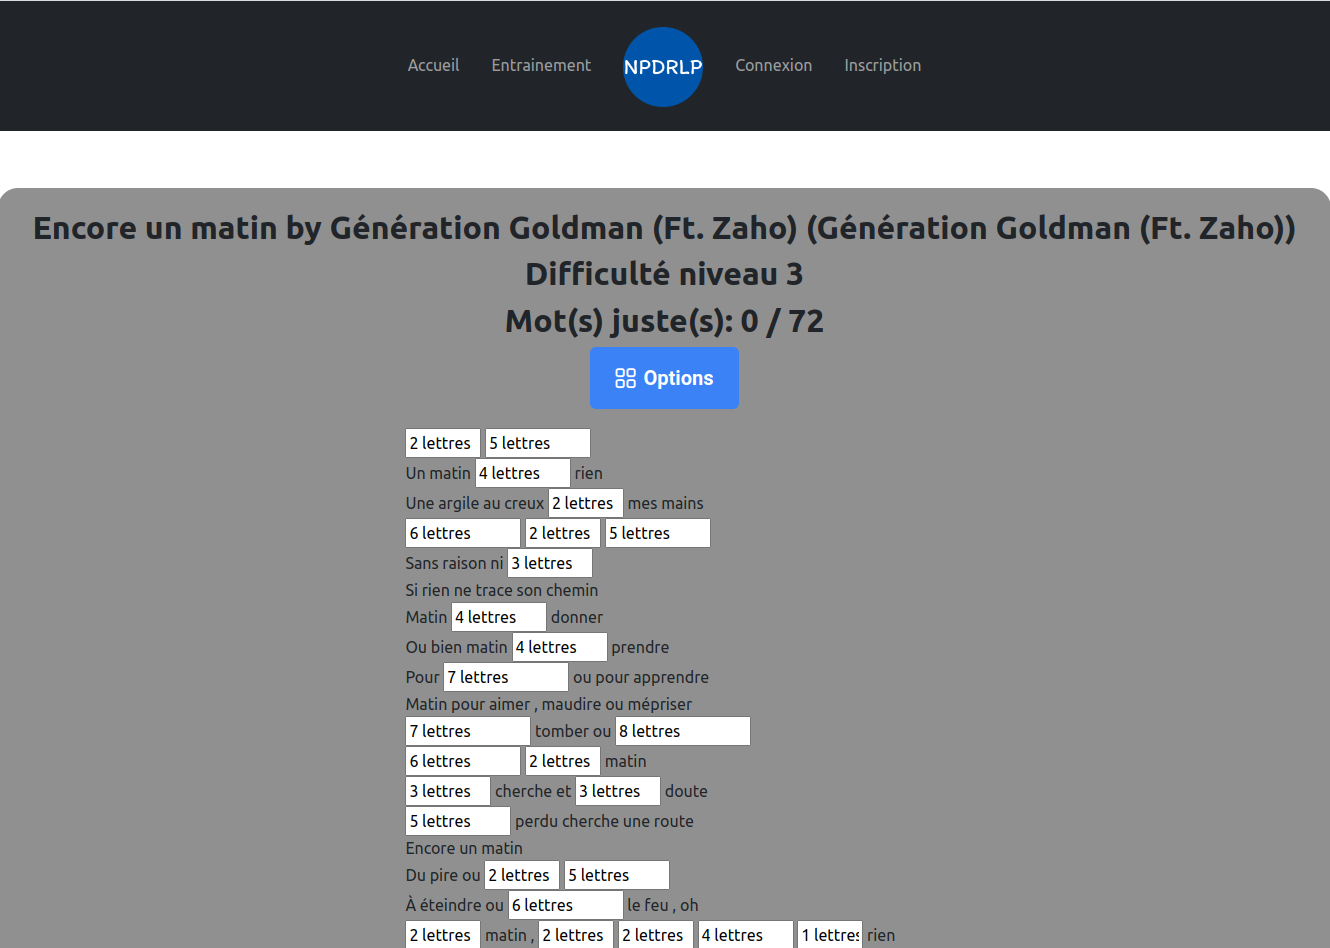
\includegraphics[scale=0.15]{diffi1.png}
	\end{minipage}%
	\begin{minipage}{.5\textwidth}
		\centering
		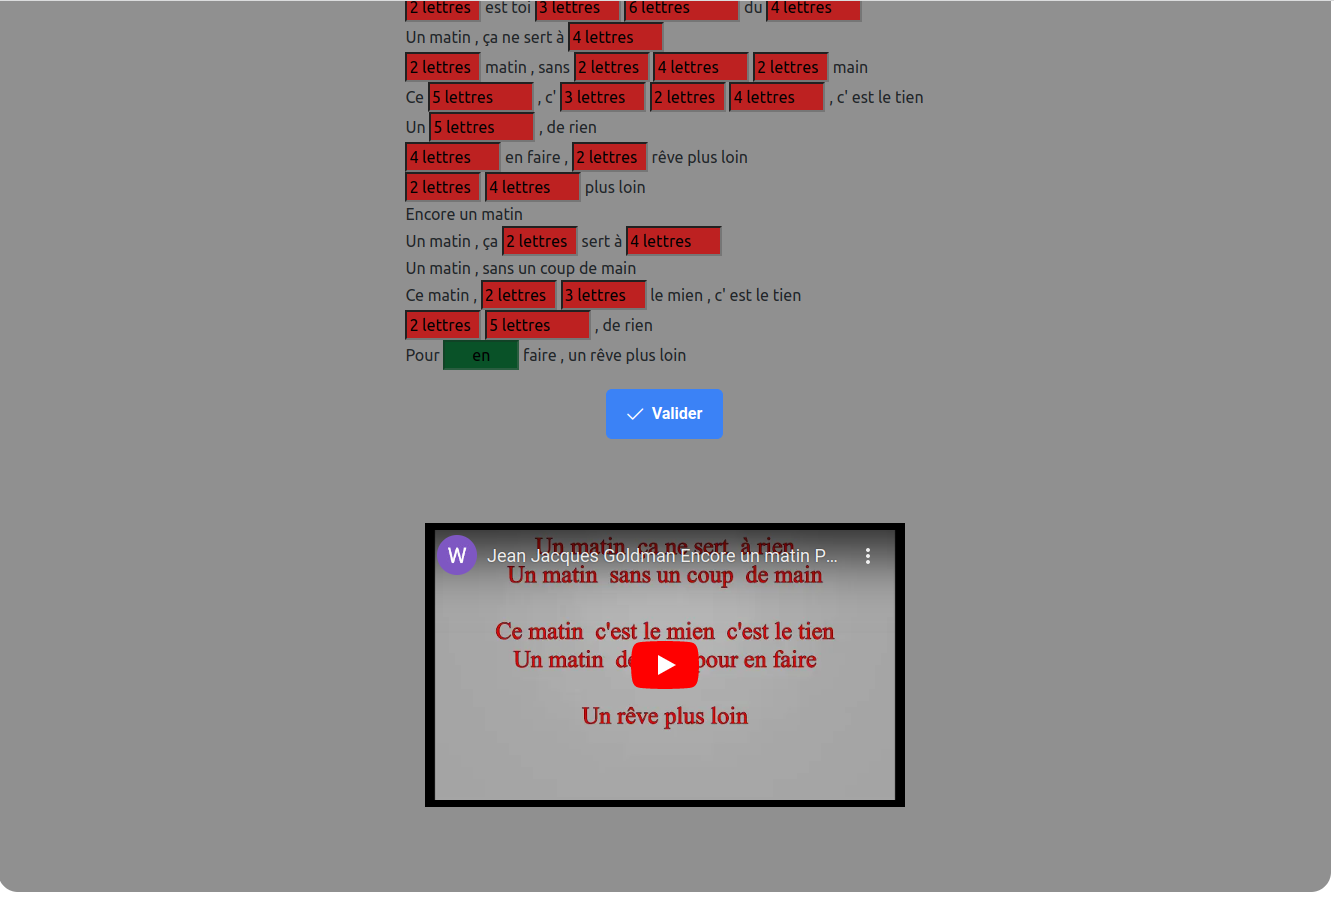
\includegraphics[scale=0.15]{diffi2.png}
	\end{minipage}
	\caption{Paroles avec des trous}
\end{figure}

\subsubsection{Inscription}

Lors de votre arrivée sur la page d'inscription, un formulaire est à remplir avec un nom d'utilisateur et une double vérification de mot de passe.

Lorsque l'utilisateur appuie sur le bouton "S'inscrire", plusieurs éléments sont vérifiés:

\begin{itemize}
	\item Nous vérifions déjà côté client que les deux mots de passe entrés sont identiques, sinon nous mettons un message d'erreur
	\item Ensuite, nous envoyons les informations au serveur. Deux retours sont alors possibles:
	\begin{itemize}
		\item Le nom d'utilisateur est déjà utilisé: on met un message d'erreur
		\item Nous avons bien enregistré le nouvel utilisateur
	\end{itemize}
\end{itemize}

\medskip

Si l'inscription a réussi, un message nous l'informe et nous sommes automatiquement redirigés vers la page de connexion après 5 secondes.

\begin{figure}[H]
	\centering
	\begin{minipage}{.5\textwidth}
		\centering
		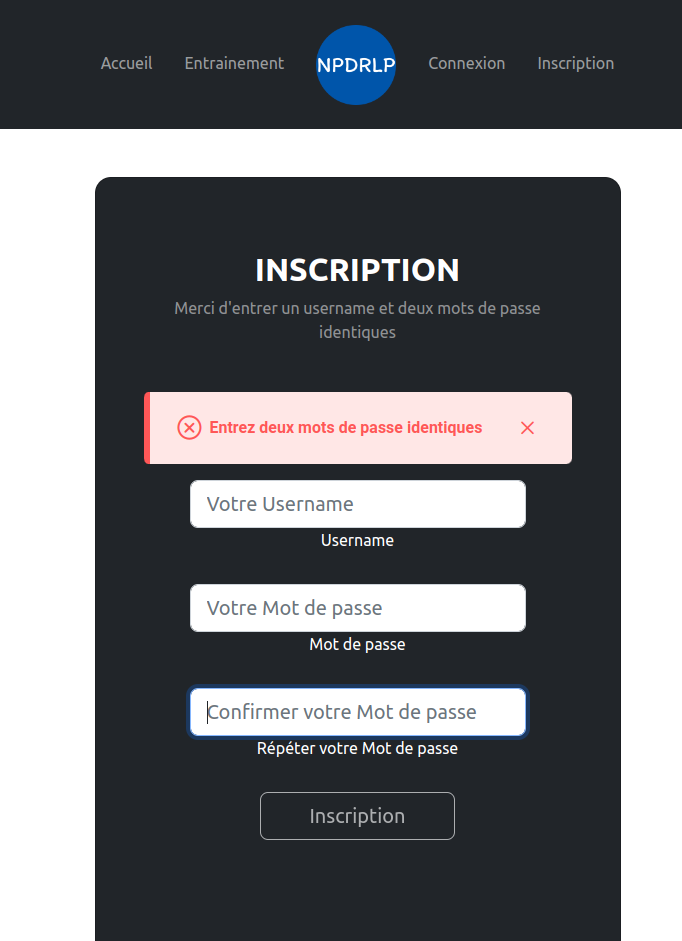
\includegraphics[scale=0.25]{inscri1.png}
	\end{minipage}%
	\begin{minipage}{.5\textwidth}
		\centering
		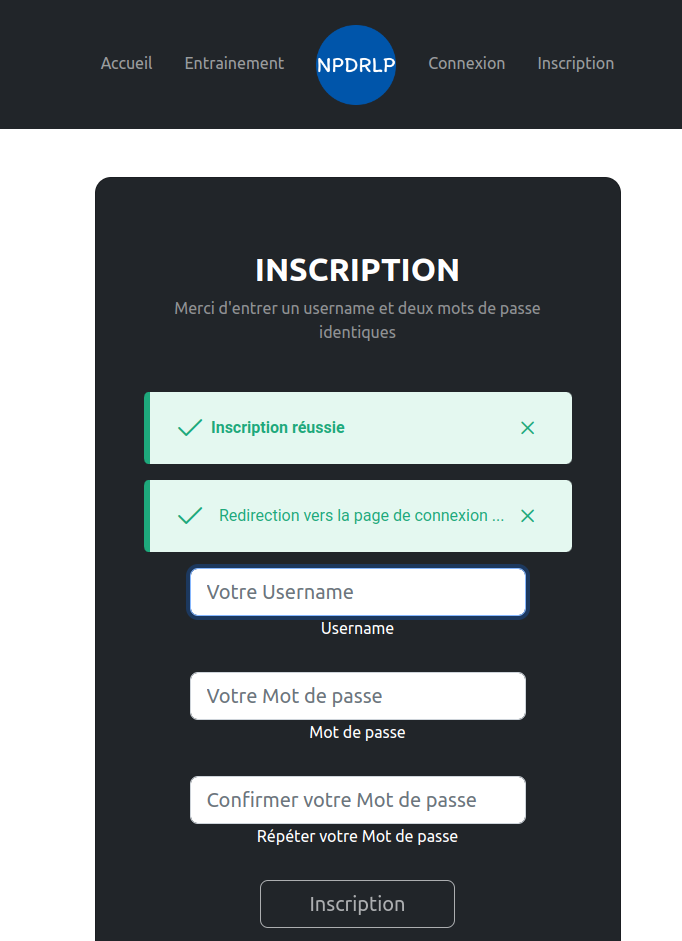
\includegraphics[scale=0.25]{inscri2.png}
	\end{minipage}
	\caption{Page d'inscription}
\end{figure}

\subsubsection{Connexion}

Nous avons ensuite la page de connexion. C'est ici que l'utilisateur, après s'être inscrit, va pouvoir débloquer l'accès à son menu personnel.

On demande de renseigner un nom d'utilisateur et le mot de passe qui va de pair avec.

Plusieurs cas d'erreur peuvent alors survenir:

\begin{itemize}
	\item Le nom d'utilisateur n'existe pas
	\item Le nom d'utilisateur existe mais le mot de passe est erroné
\end{itemize}

\medskip

Dans tous les cas, si une erreur a lieu, on empêche la connexion de l'utilisateur et on l'informe de l'erreur qui est survenue.

\begin{figure}[H]
	\centering
	\begin{minipage}{.5\textwidth}
		\centering
		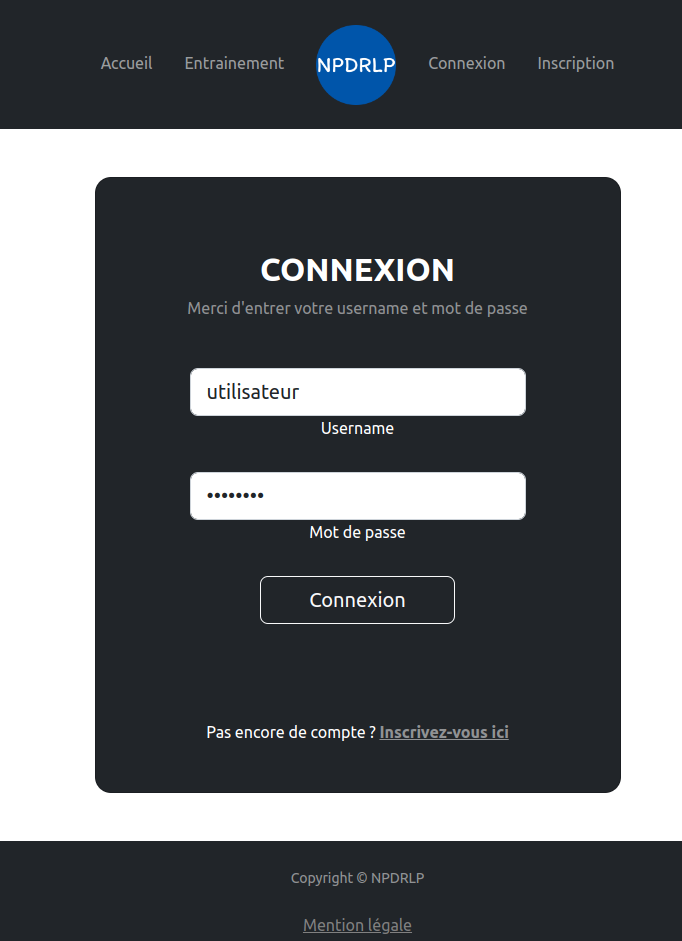
\includegraphics[scale=0.25]{connec1.png}
	\end{minipage}%
	\begin{minipage}{.5\textwidth}
		\centering
		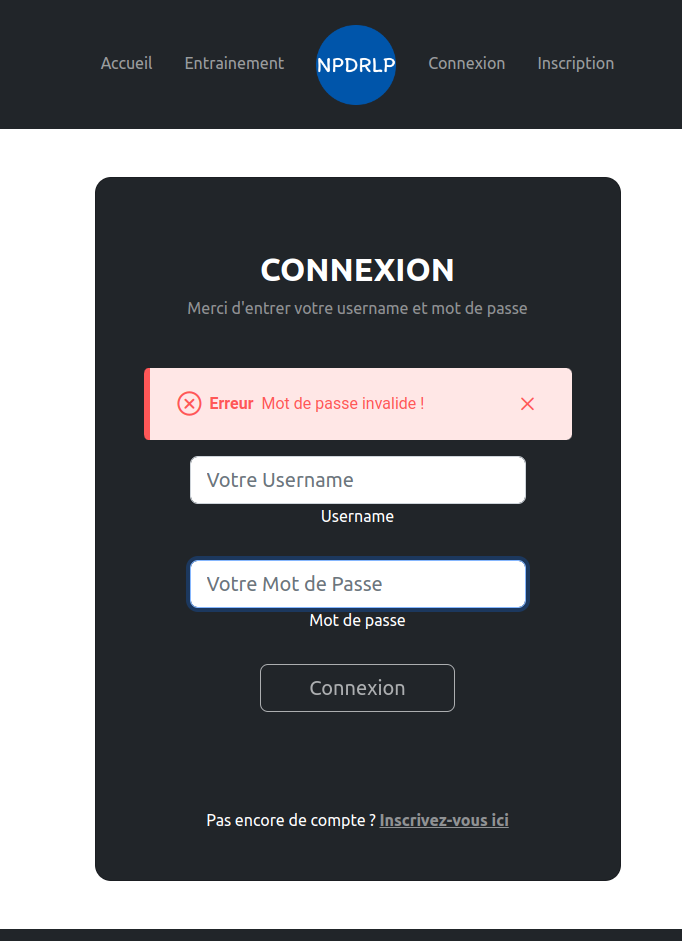
\includegraphics[scale=0.25]{connec2.png}
	\end{minipage}
	\caption{Page de connexion}
\end{figure}

Au contraire, si la connexion est réussie, on redirige automatiquement l'utilisateur vers sa page de menu. Cela arrivera quoi qu'il arrive : si jamais un utilisateur connecté essaye de retourner sur la page de connexion, nous le redirigeons directement vers son menu car il est déjà connecté !

\subsubsection{Menu de l'utilisateur}

Enfin, nous avons le menu de l'utilisateur.

Nous avons placé dedans un système d'édition de dossier ainsi qu'une explication brève et simple de comment fonctionne le site.

\begin{figure}[H]
	\centering
	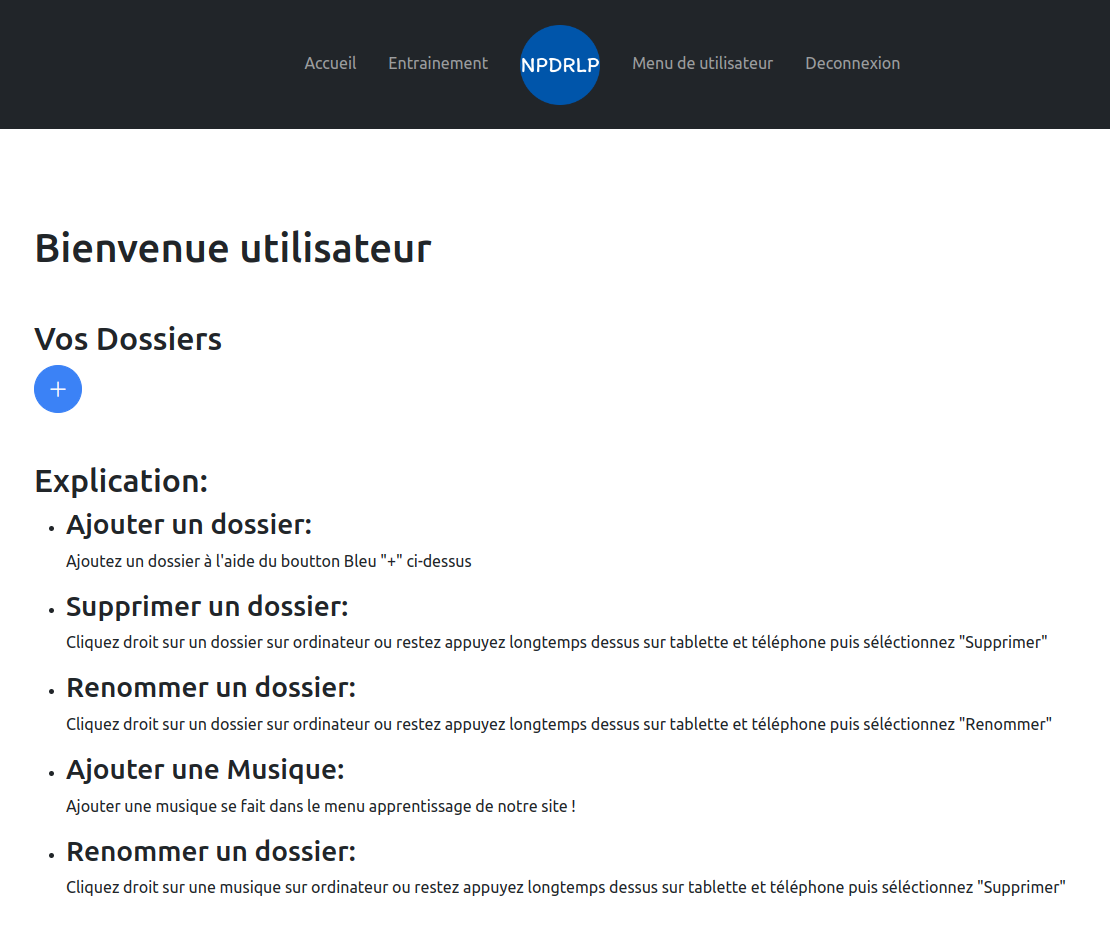
\includegraphics[scale=0.25]{menu.png}
	\caption{Le menu utilisateur}
\end{figure}

\paragraph{Le système d'édition de dossier \\\\}

À la première connexion, vous trouverez seulement un bouton avec le symbole "\textbf{+}". Ce bouton vous permet de créer un dossier avec le nom que vous voulez.

\begin{figure}[H]
	\centering
	\begin{minipage}{.5\textwidth}
		\centering
		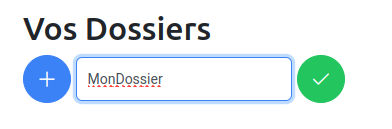
\includegraphics[scale=0.4]{dossier1.png}
	\end{minipage}%
	\begin{minipage}{.5\textwidth}
		\centering
		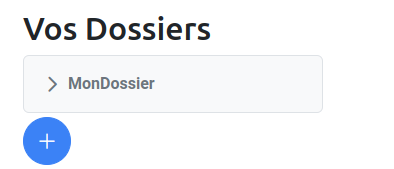
\includegraphics[scale=0.4]{dossier2.png}
	\end{minipage}
	\caption{Création d'un dossier}
\end{figure}

Vous avez ensuite la possibilité d'ajouter une musique dans un dossier comme expliqué plus tôt dans le mode entraînement.

Vous avez enfin la possibilité d'éditer vos dossiers. En faisant sur votre ordinateur un clic droit (ou un clic long sur votre téléphone et tablette) sur un dossier, vous pouvez soit le supprimer lui et toutes les musiques qui le composent, soit le renommer.

Si vous faites un clic droit sur une musique, vous pouvez la supprimer.

Avant chaque suppression d'un élément, nous demandons une confirmation à l'utilisateur car cette action est irrévocable. Une notification vous informe si votre action a bien été prise en compte ou non en haut à droite de votre écran.


\begin{figure}[H]
	\centering
	\begin{minipage}{.3\textwidth}
		\centering
		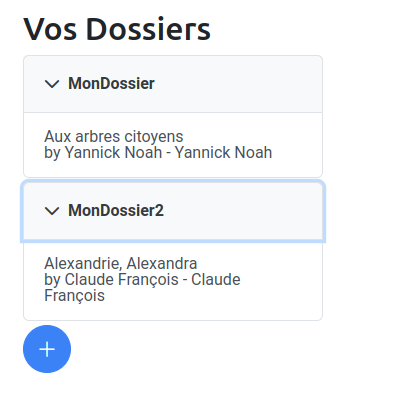
\includegraphics[scale=0.4]{dossier3.png}
	\end{minipage}%
	\begin{minipage}{.3\textwidth}
		\centering
		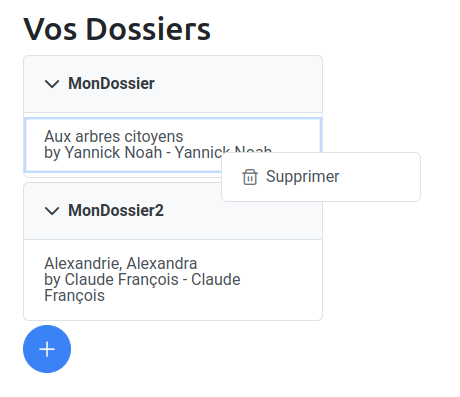
\includegraphics[scale=0.4]{dossier4.png}
	\end{minipage}
\begin{minipage}{.3\textwidth}
	\centering
	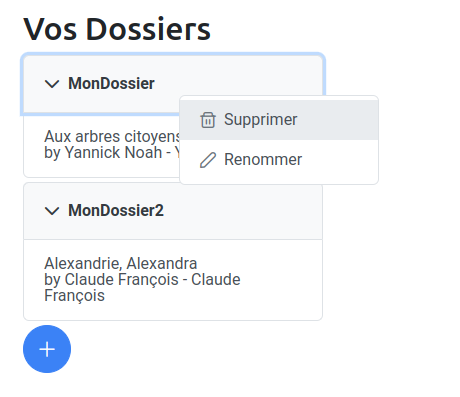
\includegraphics[scale=0.4]{dossier5.png}
\end{minipage}
	\caption{Édition des dossiers et musiques}    
\end{figure}









\end{document}
